\documentclass{article}
\usepackage[utf8]{inputenc}
\usepackage[margin = 0.8in]{geometry}
\usepackage{graphicx}
\usepackage{amsmath, amssymb}
\usepackage{subcaption}
\usepackage{multirow}
\usepackage{mathtools}
\usepackage{float}
\usepackage{enumitem}

\DeclareMathOperator*{\wrote}{Wrote}
\DeclareMathOperator*{\copyof}{CopyOf}
\DeclareMathOperator*{\owns2}{Owns}
\DeclareMathOperator*{\sings}{Sings}


\title{CS534 - HW 3}
\author{Keith Chester}
\date{Due date: July 10th 2022}

\begin{document}
\maketitle

\section*{Problem 1}

In this problem we are exploring $K$-means clustering.

We have a set of data representing five customer ratings on a new car, with a scale from 0 to 20. The image below represents that data:

\begin{figure}[H]
    \centering
    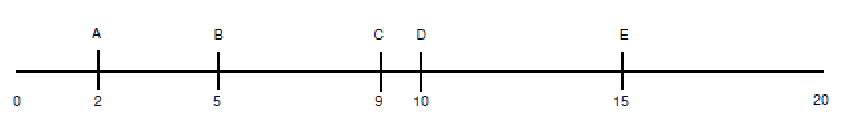
\includegraphics[width = 0.65\textwidth]{imgs/problem1_data.png}
\end{figure}

\subsection*{Part A}

Assuming that $K=2$, and the two initial centroids are $3$ and $4$, we will try to utilize the K-means algorithm to show all computational steps.

\begin{equation}
    K = [2, 5, 9, 10, 15];\; C_0 = 3;\;  C_1 = 4
\end{equation}

\noindent Next we find the distance (simple, since we're working with a singular dimension) from each point in order to assign it.

\begin{center}
    \begin{tabular}{c r r}
        Data point & Distance from $C_0$ & Distance from $C_1$\\
        2 & \textbf{1} & 2 \\
        5 & 2 & \textbf{1} \\
        9 & 6 & \textbf{5} \\
        10 & 7 & \textbf{6} \\
        15 & 12 & \textbf{11} \\
    \end{tabular}
\end{center}

\noindent Here we've bolded the closer distance to the associated centroid. We will now recompute the resulting centroid position by taking the mean value of all points assigned.

\begin{equation}
    C_i = \frac{1}{n} \sum_{x_i \rightarrow C_i} x_i
\end{equation}

\begin{equation}
    C_0 = \frac{1}{n} \sum_{x_i \rightarrow C_0} x_i = \frac{1}{1} \sum (2) = 2
\end{equation}

\begin{equation}
    C_1 = \frac{1}{n} \sum_{x_i \rightarrow C_1} x_i = \frac{1}{4} \sum (5,9,10,15) = 9.75
\end{equation}

\noindent This gives us two new centroids at $C_0=2$ and $C_1=9.75$. We continue this process until we no longer have any points change centroid assignments.

\begin{center}
    \begin{tabular}{c r r}
        Data point & Distance from $C_0$ & Distance from $C_1$\\
        2 & \textbf{0} & 7.75 \\
        5 & \textbf{3} & 4.75 \\
        9 & 7 & \textbf{0.75} \\
        10 & 8 & \textbf{0.25} \\
        15 & 13 & \textbf{5.25} \\
    \end{tabular}
\end{center}

\noindent ...since we have a new point on the first centroid, we run the calculations to get the new centroid averages again:

\begin{equation}
    C_0 = \frac{1}{n} \sum_{x_i \rightarrow C_0} x_i = \frac{1}{2} \sum (2,5) = 3.50
\end{equation}

\begin{equation}
    C_1 = \frac{1}{n} \sum_{x_i \rightarrow C_1} x_i = \frac{1}{3} \sum (9,10,15) = 11.33
\end{equation}

\noindent ...leaving us with $C_0=3.50$ and $C_1=11.33$. Continuing the process:

\begin{center}
    \begin{tabular}{c r r}
        Data point & Distance from $C_0$ & Distance from $C_1$\\
        2 & \textbf{0} & 9.33 \\
        5 & \textbf{3} & 6.333 \\
        9 & 5.50 & \textbf{2.33} \\
        10 & 6.50 & \textbf{0.67} \\
        15 & 11.50 & \textbf{3.67} \\
    \end{tabular}
\end{center}

\noindent Since we see no point changes, so our centroids are finalized at $C_0=3.50$ and $C_1=11.33$.

To find the Silhouette Coefficient Index, we take a given cluster $C_i$, select a point $x_i$ within it, and find the average distance distance between it and all other points within that cluster, which we'll mark as $a_1$. Then for each other cluster $C_j$, find the \textit{minimum} average distance ($a_j$) between this point and the average distance from each point in the other clusters.

\noindent ...choosing $x_i=x_0=2$ for our point

\begin{equation}
    a_1 = 3
\end{equation}

/noindent ...we need to test both $x_0$ and $x_1$ to find the minimum average distance to utilize for our calculation.

\begin{equation}
    a_2 = \frac{1}{n} \sum d(x_0, C_1); \; = \frac{1}{3} (7, 8, 13) = 9.33
\end{equation}

\begin{equation}
    a_2 = \frac{1}{n} \sum d(x_1, C_1); \; = \frac{1}{3} (4, 5, 10) = 6.33
\end{equation}


\noindent ...which, since we have only the one other cluster, we can stop here. We'll use the smaller $6.33$ average distance. If we had more clusters, we would take the minimum of the average distances from each point in other clusters, but we can stop here. We can now calculate the index $S_1$:

\begin{equation}
    S_1 = 1 - \frac{a_1}{a_2} = 1 - \frac{3}{6.33} = 0.53
\end{equation}

\noindent ...and then we do the same for the next cluster $C_2$. We use $x_i=x_3=9$.

\begin{equation}
    a_1 = \frac{1}{n} \sum d(x_2, C_1); \; = \frac{1}{2} (1, 6) = 3.5
\end{equation}

/noindent ...we need to test both $x_2$, $x_3$ and $x_4$ to find the minimum average distance to utilize for our calculation.

\begin{equation}
    a_2 = \frac{1}{n} \sum d(x_2, C_0); \; = \frac{1}{2} (7, 4) = 5.5
\end{equation}

\begin{equation}
    a_2 = \frac{1}{n} \sum d(x_3, C_0); \; = \frac{1}{2} (8, 5) = 6.5
\end{equation}

\begin{equation}
    a_2 = \frac{1}{n} \sum d(x_4, C_0); \; = \frac{1}{2} (12, 10) = 11
\end{equation}

\noindent ...using $a_2=5.5$ as our minimum.

\begin{equation}
    S_2 = 1- \frac{a_1}{a_2} = 1 - \frac{3.5}{5.5} = 0.37
\end{equation}

\noindent ...so the Silhouette Coefficient Index for our clusters $C_0$ and $C_1$ are $S_1=0.76$ and $S_2=0.37$, respectively.

\end{document}